\documentclass{beamer}

\usepackage[utf8]{inputenc}
\usepackage[T1]{fontenc}
\usepackage{textcomp}
\usepackage{times}

\usetheme{Frankfurt}
\usecolortheme{orchid}

\usepackage{color}

\title{How social media affect FOSS}
\subtitle{INF5780 Project 2}
\author{{John Rongved} \and {Lars Tveito} \and {Kristian A. Hiorth}}
\date{November 13, 2014}

\institute{Department of Informatics\\University of Oslo}

% fits the presentation to the window when first displayed
\hypersetup{pdfstartview={Fit}}

\AtBeginSubsection[]
{
  \begin{frame}<beamer>{Outline}
    \tableofcontents[currentsection,currentsubsection]
  \end{frame}
}

\newcommand{\coloreddot}[1][black]{\Large\textcolor{#1}{\ensuremath\bullet}}
\setbeamertemplate{caption}{\raggedright\insertcaption\par}

\begin{document}


\begin{frame}
  \titlepage
\end{frame}

\begin{frame}{Outline}
  \tableofcontents{}
\end{frame}

\section{Motivation}

\subsection{Research Topic}

\begin{frame}
  \frametitle{Research Topic}
  \begin{itemize}
  \item Free and Open Source Software (FOSS) projects are a kind of Community
    Based Peer Production (CBPP)
  \item They revolve around a community
  \item Social Media has changed how Internet
    communities work

    \pause

  \item We wanted to investigate how Social Media have been, and are,
    influencing FOSS projects in particular
  \end{itemize}
\end{frame}

\subsection{Key Aspects of FOSS Projects}

\begin{frame}{Key Aspects}{Attention}
  FOSS projects need to communicate wit
\end{frame}

\begin{frame}{Key Aspects}{Support}
\end{frame}

\begin{frame}{Key Aspects}{Development Tools}
\end{frame}

\subsection{Key Social Media Sites}

\begin{frame}
  \frametitle{GitHub vs Sourceforge}
  \begin{figure}
    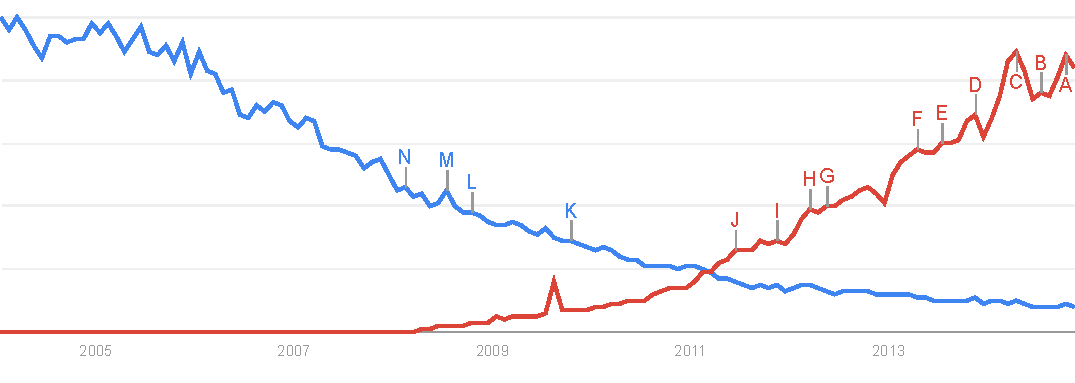
\includegraphics[width=\textwidth]{sourceforge-github.pdf} \\
    \caption{\coloreddot[red] Github \hspace{2em} \coloreddot[blue] Sourceforge}
    \end{figure}
\end{frame}



\begin{frame}
  \frametitle{Social News}

  \begin{center}
    
\includegraphics[width=.6\textwidth]{Reddit_logo.pdf}

  \vskip0pt plus.5fill

    
\includegraphics[width=.6\textwidth]{hacker-news_logo.jpg}
  \end{center}

\end{frame}


\begin{frame}{Social Q \& A}
  \begin{center}
    
\includegraphics[width=.6\textwidth]{so-logo.eps}
  \end{center}
\end{frame}

\begin{frame}{Social Coding}
  \begin{center}
    
\includegraphics[width=.6\textwidth]{GitHub_Logo.eps}
  \end{center}
\end{frame}

\section{Related work}

\subsection{Social coding}


\subsection{Social Q \&{} A}

\subsection{Social news}


\section{Discussion}

\subsection{Shizz}

\begin{frame}
  Shoozial mediaz da bomb, man.
\end{frame}

\section*{Summary}

\begin{frame}
  We showed dem mediaz be sozial.

  
  \pause
  \vskip0pt plus.5fill

  Questions?
\end{frame}

\end{document}
